\input{header.tex}

\subject{V46}
\title{Der Faraday-Effekt an Halbleitern}
\date{%
  Durchführung: 13.05.2026
  \hspace{3em}
  Abgabe: DATUM
}

\mathtoolsset{showonlyrefs}

\begin{document}

\maketitle
\thispagestyle{empty}
\tableofcontents
\newpage

\section{Zielsetzung}
\label{sec:zielsetzung}

Ziel des Versuchs ist es die Faraday-Rotation an unterschiedlich dotierten GaAs-Halbleitern zu untersuchen und dadurch die effektive Masse der Ladungsträger zu bestimmen. 
\section{Theorie}
\label{sec:Theorie}

\subsection{Glan-Thompson-Prisma}

\clearpage
\section{Durchführung}
\label{sec:Durchführung}

\begin{figure}[htbp]
    \centering
    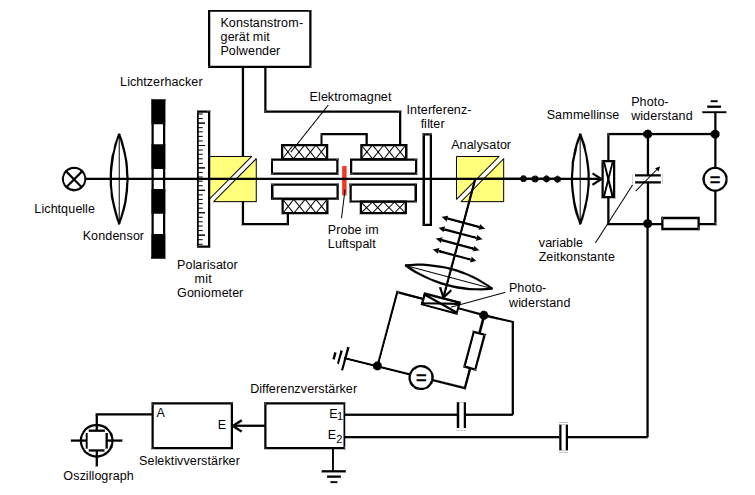
\includegraphics[width=0.8\textwidth]{content/pics/aufbau.png}
    \caption{Darstellung des Versuchsaufbaus.~\cite{Durchfuhrung}}
    \label{fig:aufbau}
\end{figure}

\clearpage
\section{Auswertung}
\label{sec:Auswertung}

% Fehlerrechnung
Die in diesem Kapitel durchgeführten Fehlerrechnungen wurden mittels der Gaußschen Fehlerfortpflanzung 
\begin{equation}
    \sigma_f = \sqrt{\left( \frac{\partial f}{\partial x_1} \sigma_{x_1} \right)^2 + \left( \frac{\partial f}{\partial x_2} \sigma_{x_2} \right)^2 + ...}
\end{equation}
durchgeführt, sowie den Formeln 
\begin{equation}
    \overline{x} = \frac{1}{n} \sum^n_{i=1}x_i . 
    \label{eq:mittelwert}
\end{equation}
für den Mittelwert und 
\begin{equation}
    \sigma_{\overline{x}} = \frac{\sigma_x}{\sqrt{n}} = \sqrt{\frac{1}{n(n-1)}  \sum^n_{i=1} \left( x_i - \overline{x}\right)^2 } .
    \label{eq:abweichung}
\end{equation}
für die Standardabweichung einer Messreihe $\left( x_1, ... , x_n  \right)$.
Der Einfachheit halber wird hierbei das Python-Paket \textit{uncertainties} verwendet. \cite{uncertainties} \\
\hspace{1cm}
% Ende Fehlerrechnung

\subsection{Bestimmung des B-Feldes}
Im Folgenden sind die Messwerte zur Bestimmung des B-Feldes aufgetragen.

\begin{table}[H]
    \centering
    \caption{Messwerte der magnetischen Kraftflussdichte entlang der z-Achse}
    \label{tab:magnetfeld}
    \begin{tabular}{rrr}
        \toprule
        \textbf{$B$ [mT]} & \textbf{$x$ [mm]} & \textbf{$x_{\text{rel}}$ [mm]} \\
        \midrule
        159 & 103 &  12 \\
        202 & 104 &  11 \\
        245 & 105 &  10 \\
        285 & 106 &   9 \\
        319 & 107 &   8 \\
        346 & 108 &   7 \\
        366 & 109 &   6 \\
        381 & 110 &   5 \\
        391 & 111 &   4 \\
        399 & 112 &   3 \\
        404 & 113 &   2 \\
        406 & 114 &   1 \\
        410 & 115 &   0 \\
        408 & 116 &  -1 \\
        406 & 117 &  -2 \\
        400 & 118 &  -3 \\
        393 & 119 &  -4 \\
        382 & 120 &  -5 \\
        367 & 121 &  -6 \\
        348 & 122 &  -7 \\
        323 & 123 &  -8 \\
        292 & 124 &  -9 \\
        254 & 125 & -10 \\
        212 & 126 & -11 \\
        \bottomrule
    \end{tabular}
\end{table}

Zur Bestimmung des maximalen B-Feldes, also dem B-Feld in dem unsere Proben sitzen wird, werden die Punkte aufgetragen und es wird graphisch ein Maximum bestimmt.
\begin{figure}[H]
    \centering
    
\includegraphics[width=0.8\textwidth]{content/plots/Bfeld.png}
    \caption{B-Feld in Abhängigkeit des Ortes..}
    \label{fig:B-Feld}
\end{figure}

\subsection{Drehwinkel der Proben}

Im Folgenden sind die Messwerte zur Bestimmung der Drehwinkel der Proben aufgetragen.

\begin{table}[htpb]
    \centering
    \caption{Messdaten für die Rotationswinkel für je zwei Polrichtungen des Magnetfeldes $B$, für 3 verschiedene Proben bei verschiedenen Wellenlängen.}
    \label{tab:rotationswinkel}
    \begin{tabular}{lcccccc}
        \toprule
        & \multicolumn{2}{c}{Probe 1 (undotiert)} & \multicolumn{2}{c}{Probe 2 (n-dotiert 1)} & \multicolumn{2}{c}{Probe 3 (n-dotiert 2)} \\
        \cmidrule(lr){2-3} \cmidrule(lr){4-5} \cmidrule(lr){6-7}
        $\lambda/\mathrm{\mu m}$ & $\theta_1$ & $\theta_2$ & $\theta_1$ & $\theta_2$ & $\theta_1$ & $\theta_2$ \\
        \midrule
        1,06  & $164^\circ 09'$ & $140^\circ 36'$ & $255^\circ 35'$ & $264^\circ 15'$ & $256^\circ 55'$ & $264^\circ 51'$ \\
        1,29  & $159^\circ 44'$ & $144^\circ 11'$ & $263^\circ 52'$ & $255^\circ 34'$ & $257^\circ 00'$ & $262^\circ 22'$ \\
        1,45  & $155^\circ 53'$ & $146^\circ 09'$ & $265^\circ 01'$ & $257^\circ 00'$ & $259^\circ 09'$ & $264^\circ 54'$ \\
        1,72  & $83^\circ 45'$  & $76^\circ 35'$  & $157^\circ 05'$ & $147^\circ 53'$ & $257^\circ 42'$ & $262^\circ 41'$ \\
        1,96  & $79^\circ 11'$  & $73^\circ 55'$  & $161^\circ 28'$ & $150^\circ 15'$ & $253^\circ 34'$ & $258^\circ 54'$ \\
        2,156 & $77^\circ 23'$  & $72^\circ 04'$  & $164^\circ 10'$ & $152^\circ 01'$ & $251^\circ 14'$ & $258^\circ 39'$ \\
        2,34  & $51^\circ 43'$  & $47^\circ 39'$  & $189^\circ 01'$ & $176^\circ 00'$ & $226^\circ 00'$ & $233^\circ 11'$ \\
        2,51  & $33^\circ 30'$  & $30^\circ 29'$  & $207^\circ 29'$ & $192^\circ 03'$ & $207^\circ 04'$ & $216^\circ 55'$ \\
        2,65  & $347^\circ 24'$ & $341^\circ 15'$ & $169^\circ 00'$ & $156^\circ 26'$ & $244^\circ 40'$ & $253^\circ 01'$ \\
        \bottomrule
    \end{tabular}
\end{table}

Im Folgenden werden die Drehwinkel für die drei Proben in Abhängigkeit der Wellenlänge graphisch aufgetragen. 


\begin{figure}[H]
    \centering
    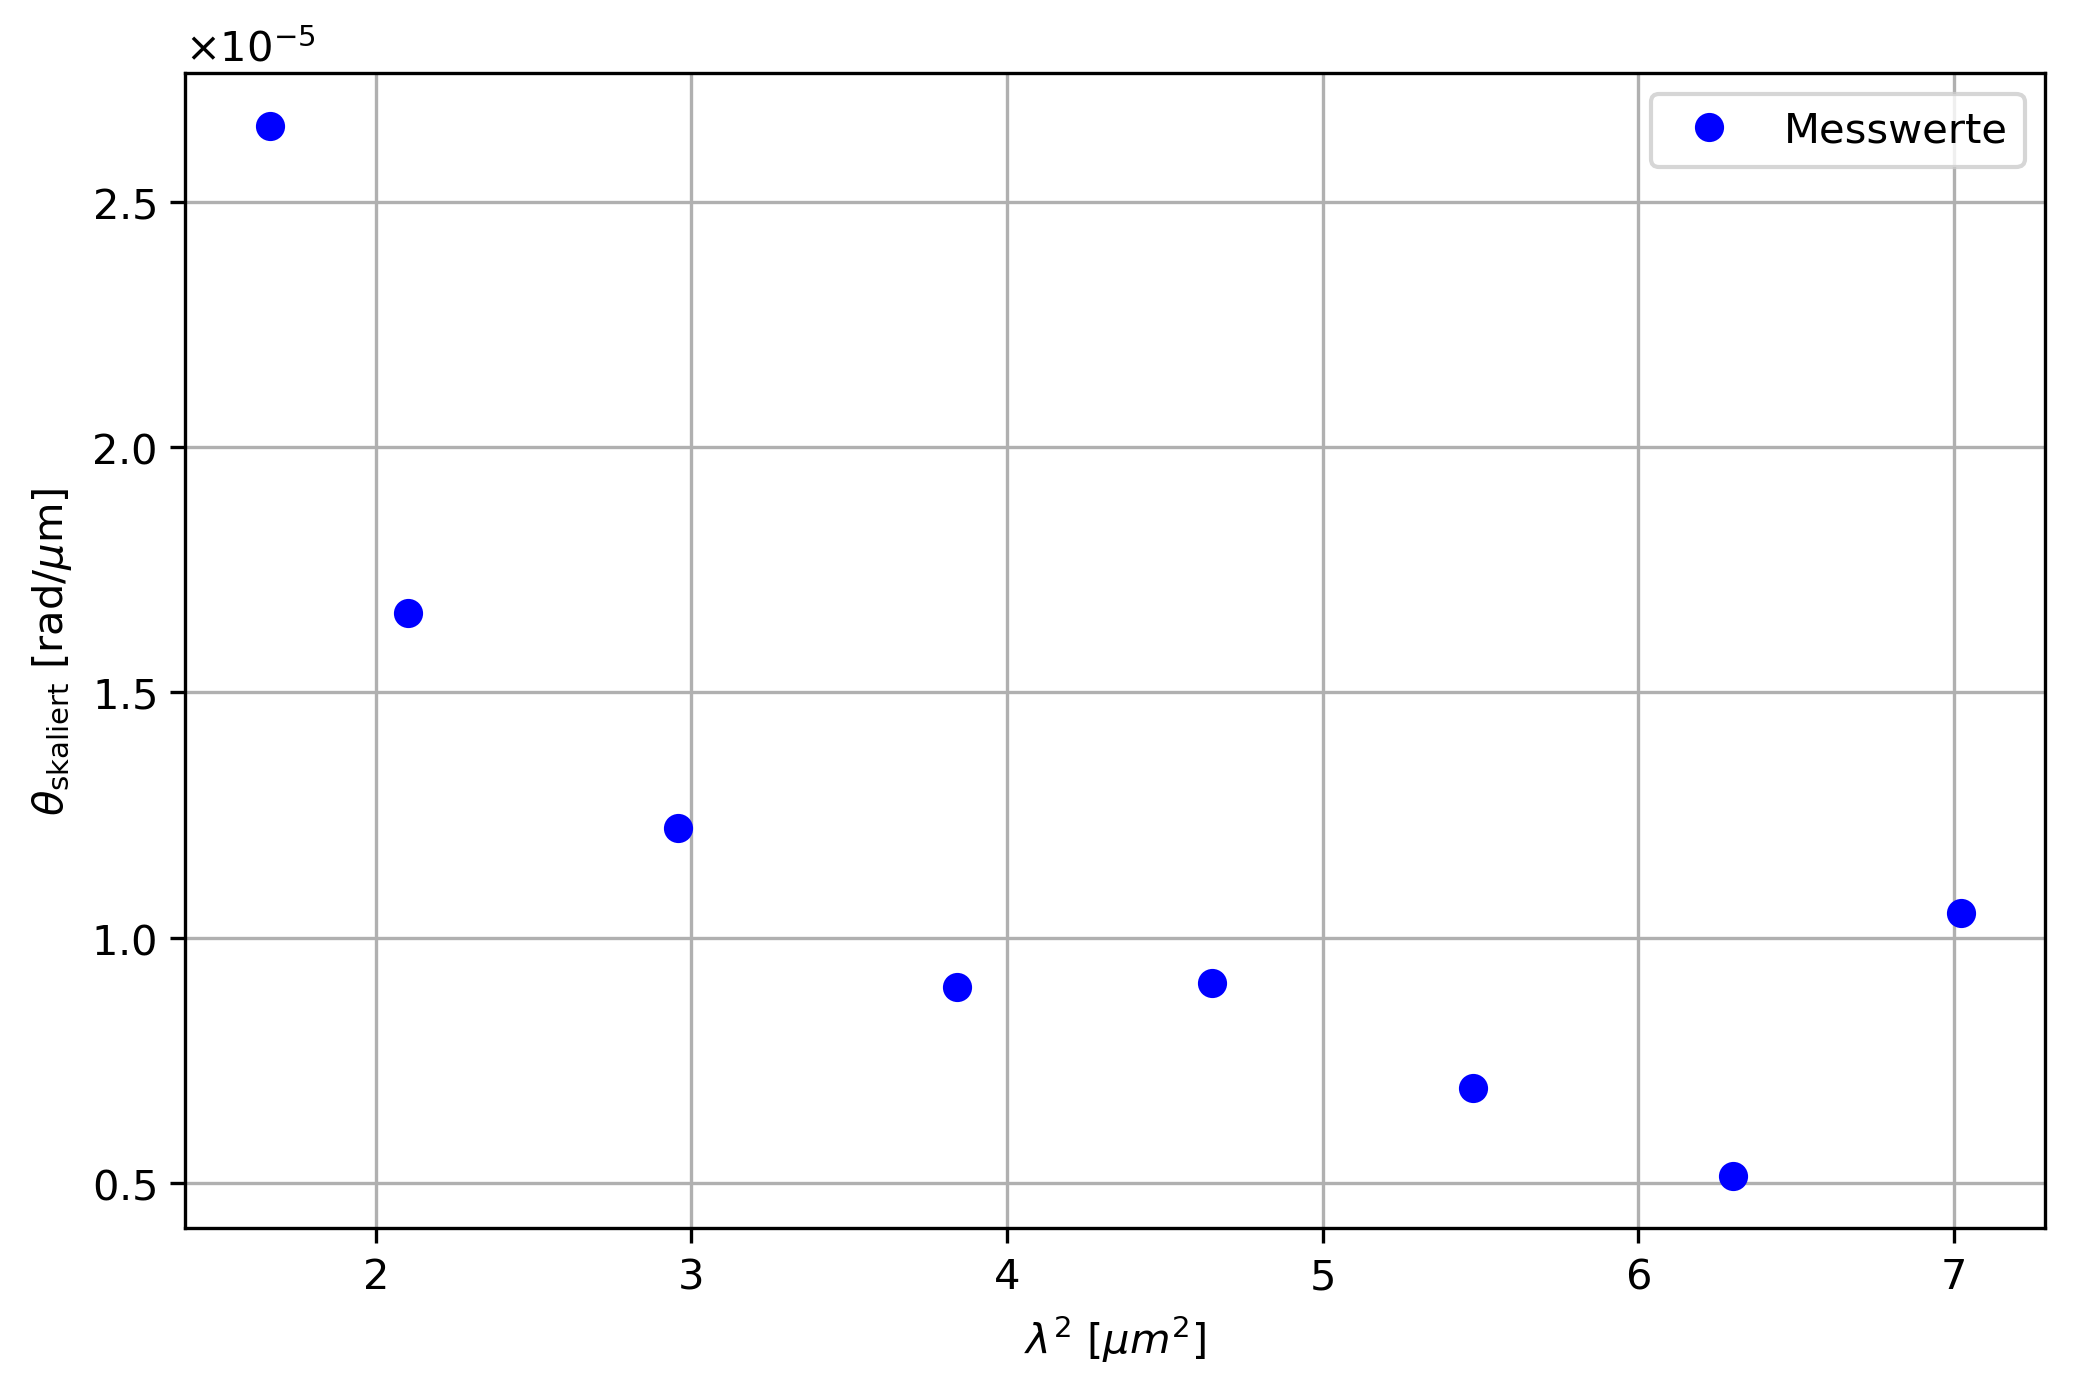
\includegraphics[width=0.8\textwidth]{content/plots/theta_vs_lambda_undotiert.png}
    \caption{Drehwinkel der undotierten Probe in Abhängigkeit der Wellenlänge.}
\end{figure}

\begin{figure}[H]
    \centering
    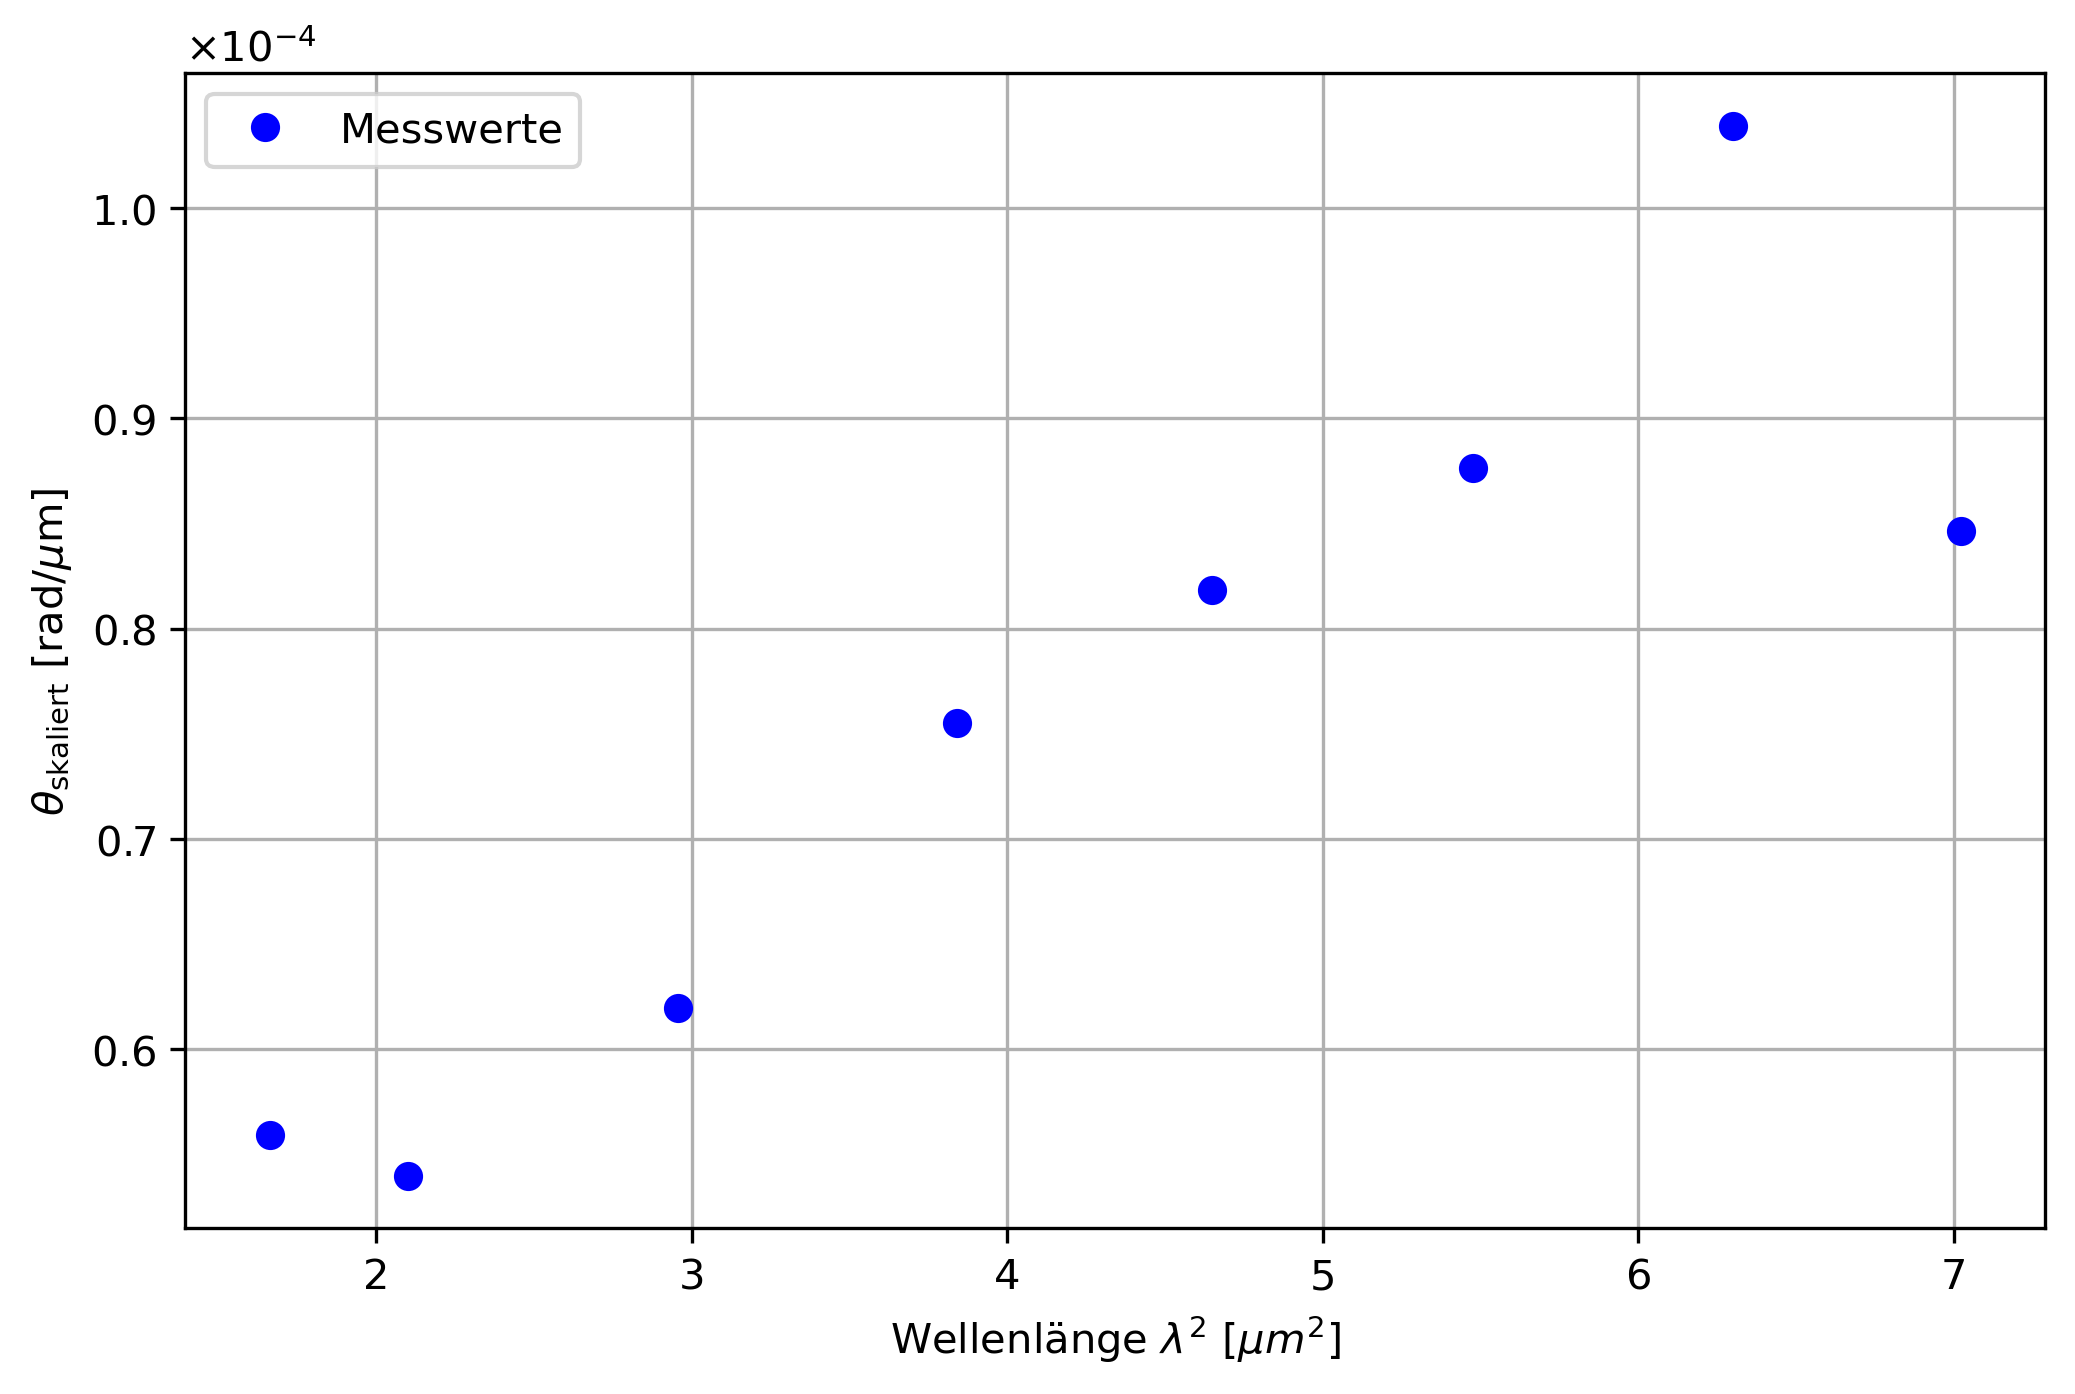
\includegraphics[width=0.8\textwidth]{content/plots/theta_vs_lambda_n1.png}
    \caption{Drehwinkel der ersten n-dotierter Probe in Abhängigkeit der Wellenlänge.}
\end{figure}

\begin{figure}[H]
    \centering
    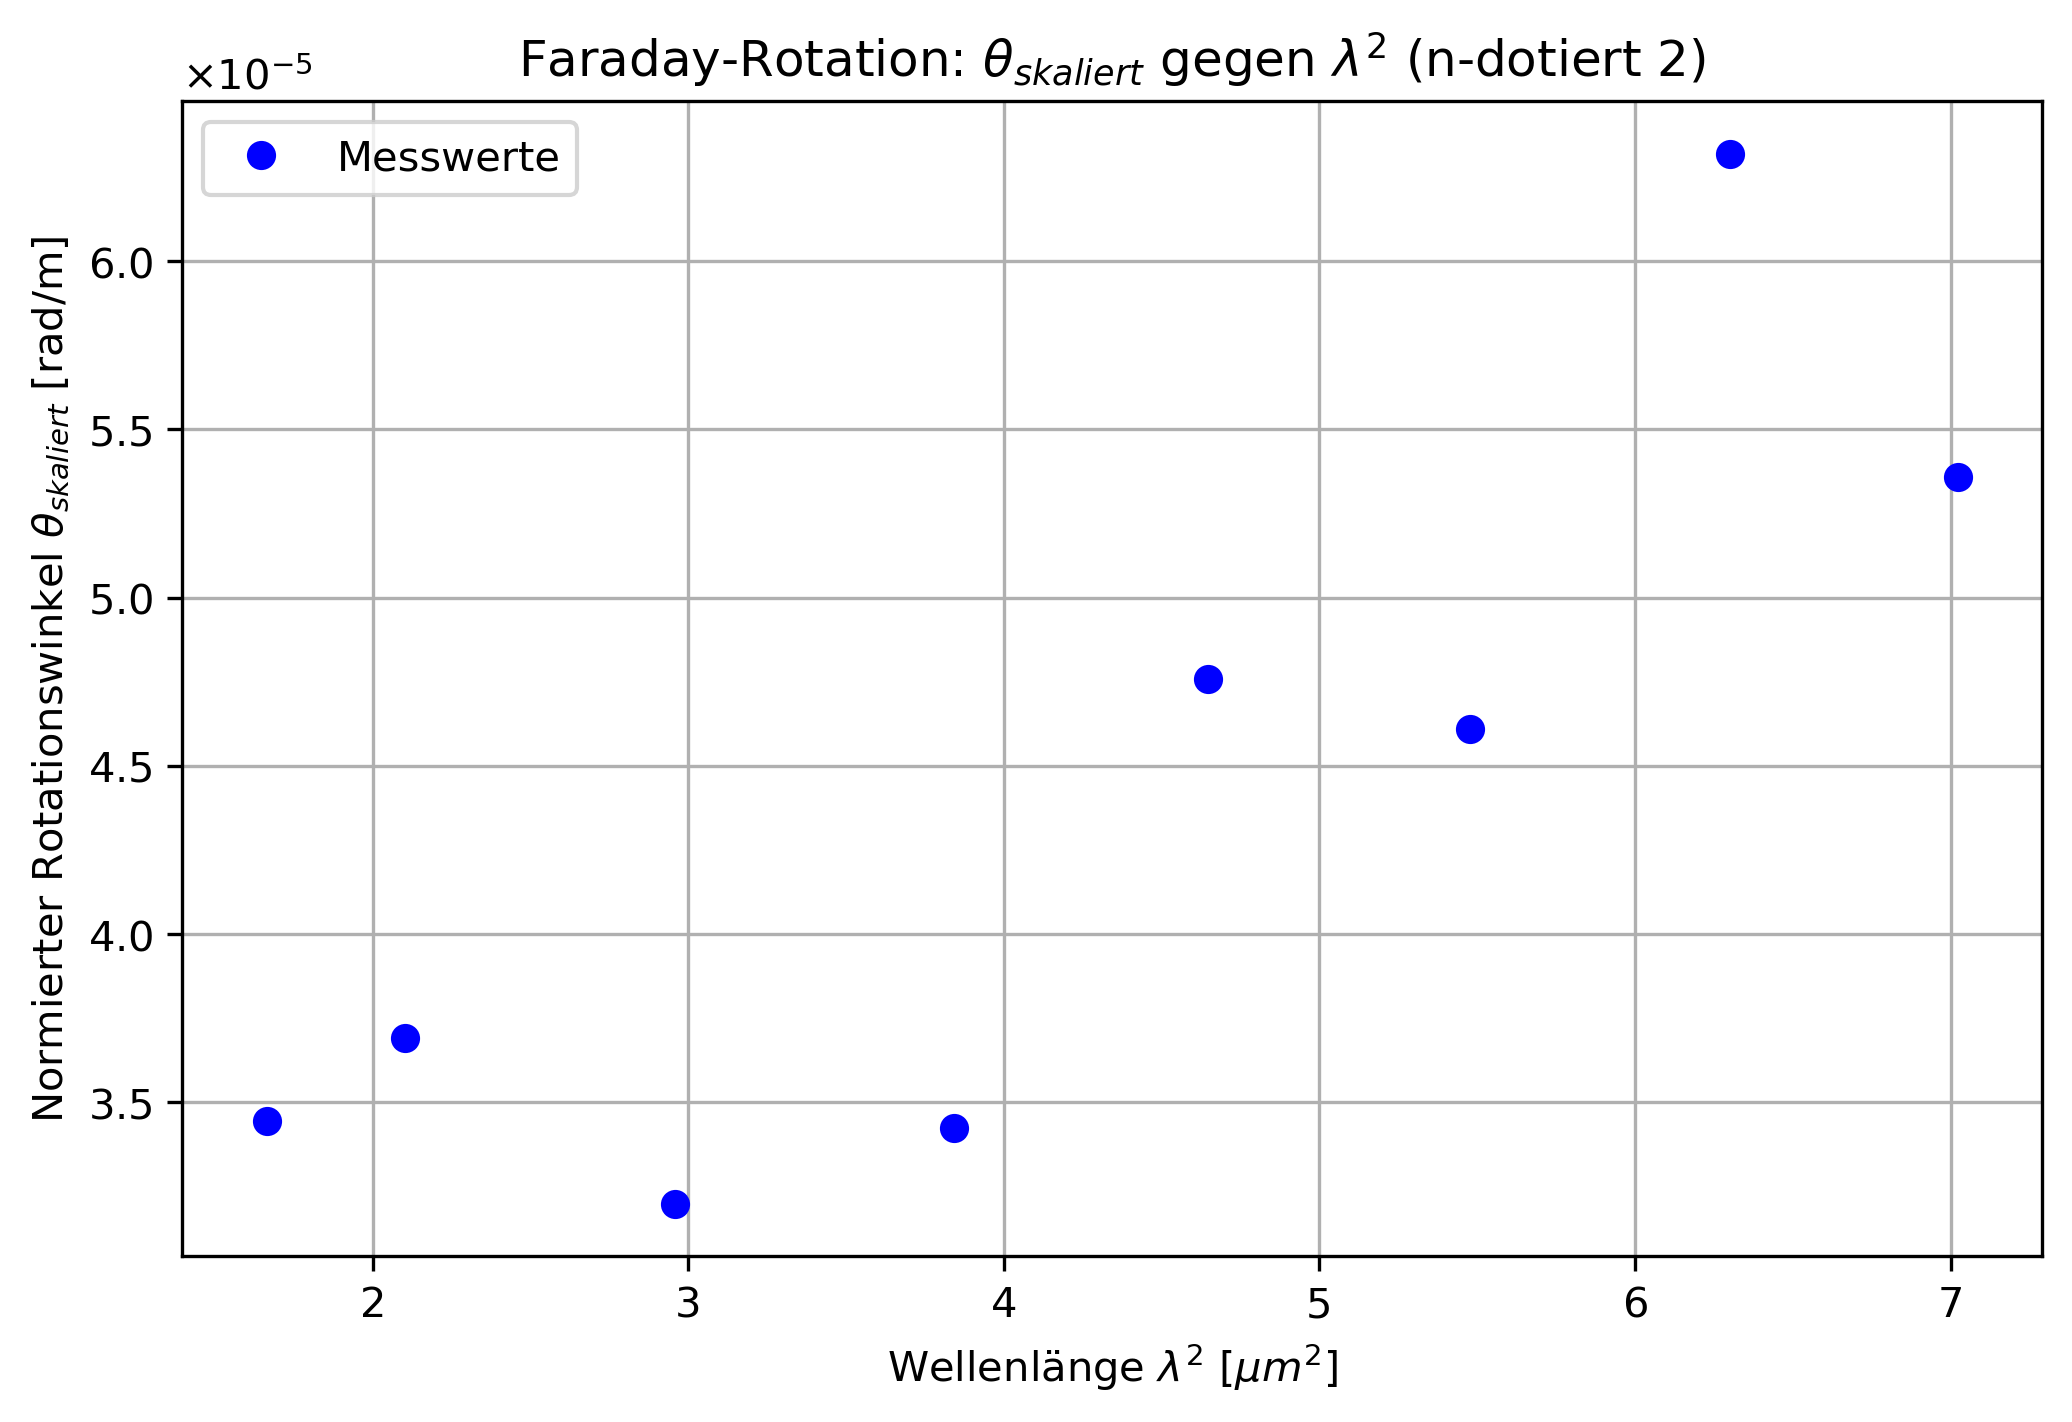
\includegraphics[width=0.8\textwidth]{content/plots/theta_vs_lambda_n2.png}
    \caption{Drehwinkel der zweiten n-dotierter Probe in Abhängigkeit der Wellenlänge.}
\end{figure}
\subsection{Bestimmung der effektiven Masse}
Im Folgenden wird der die Differenz der n-dotierten Proben zu der undotierten Probe gebildet, um die effektive Masse zu bestimmen.

\begin{figure}[H]
    \centering
    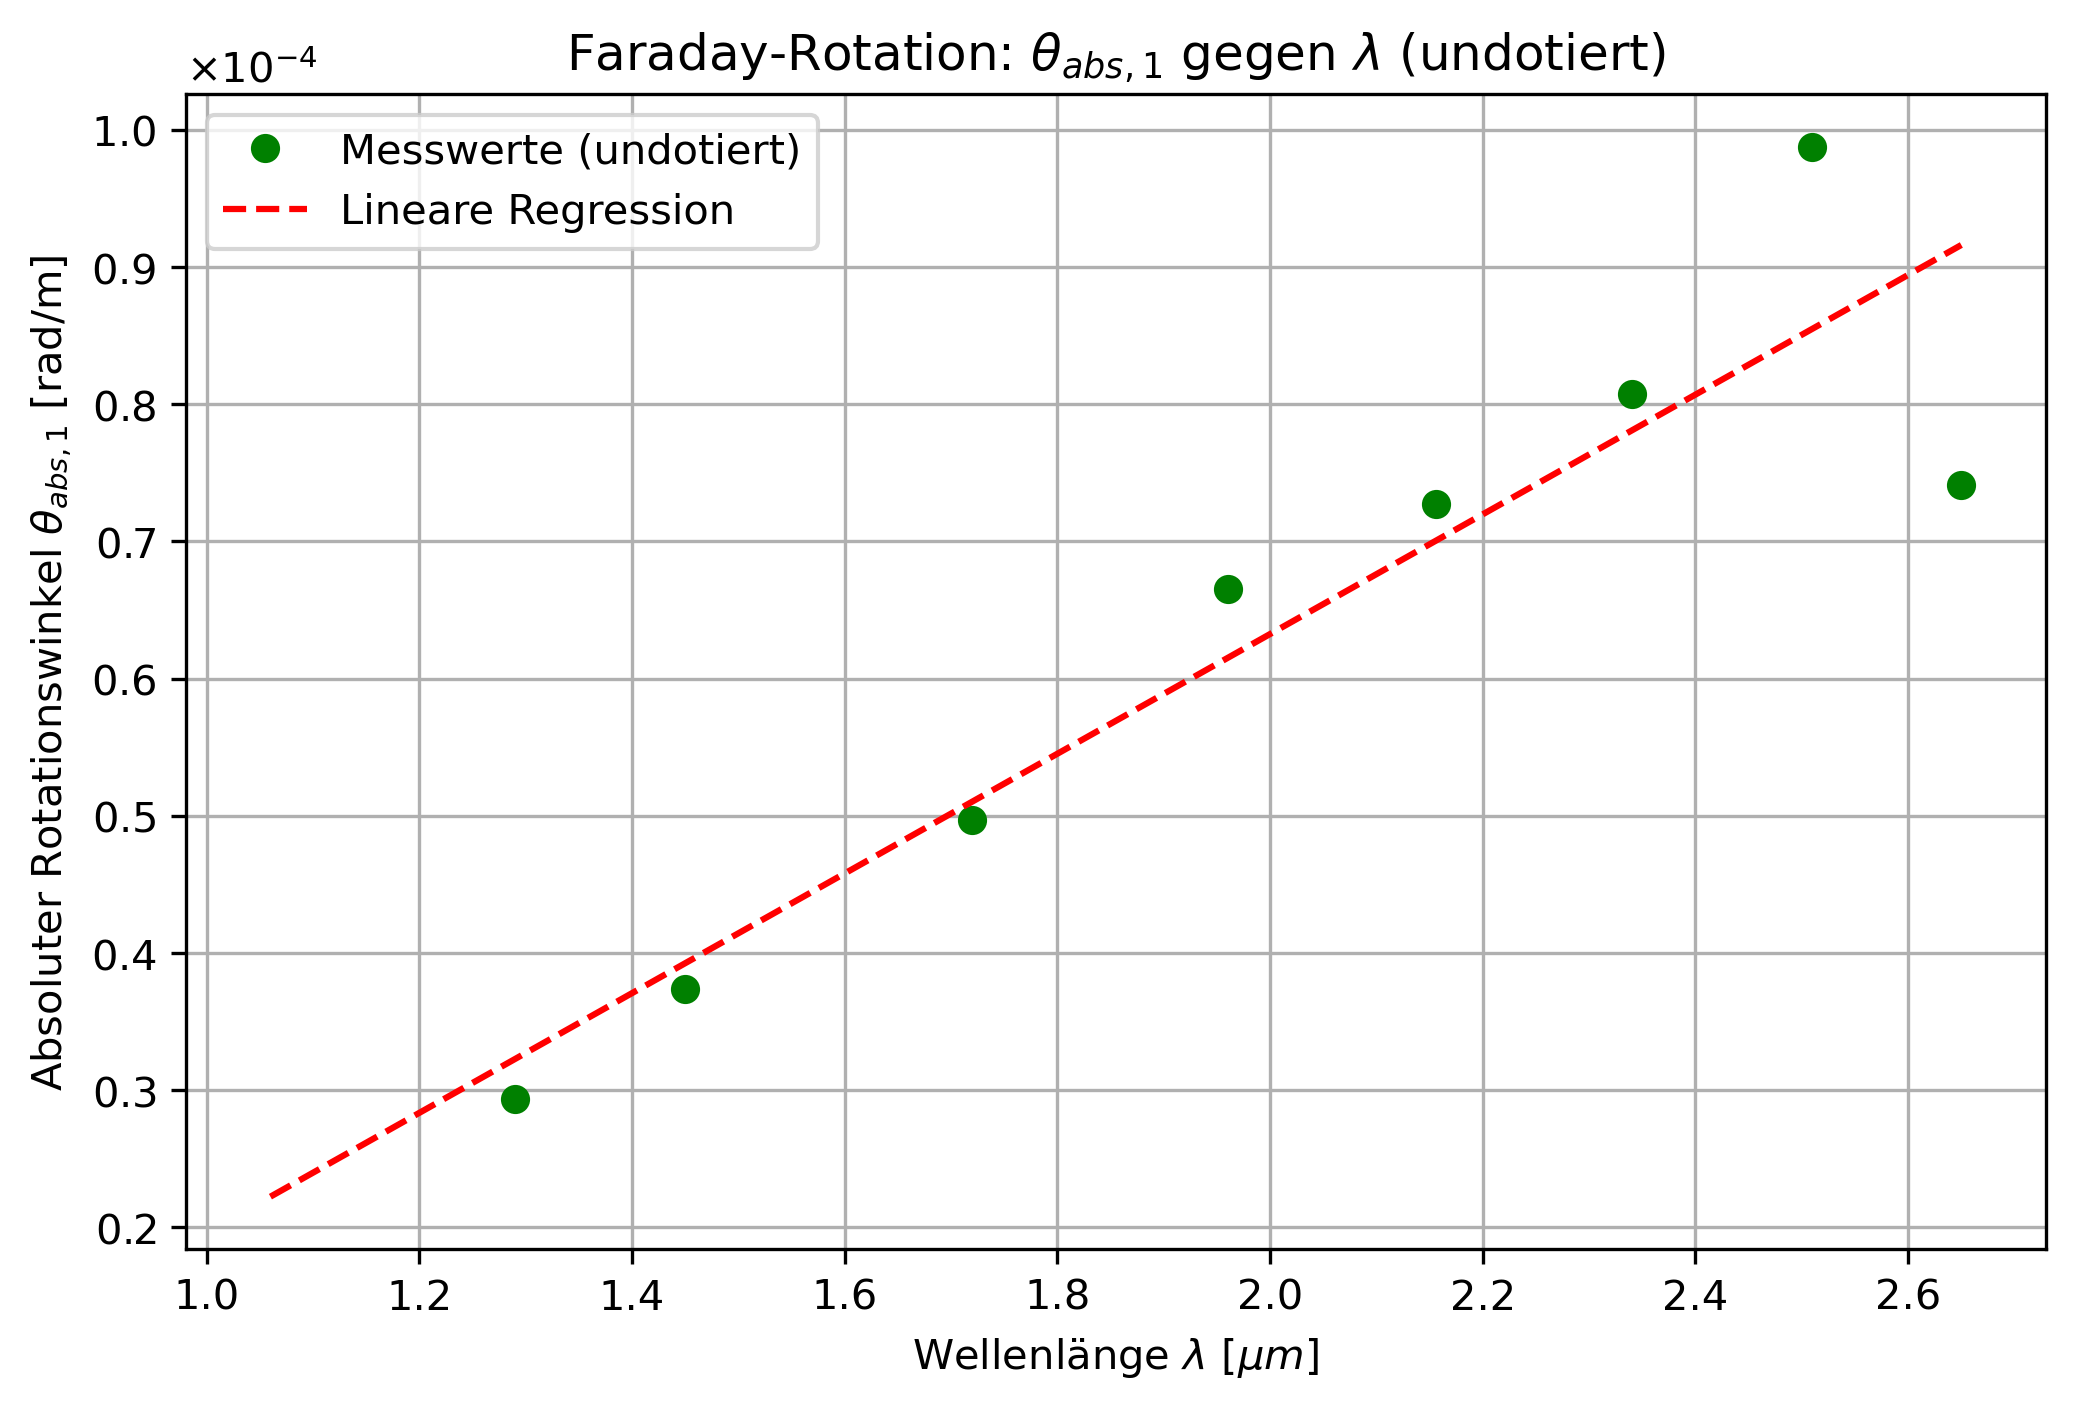
\includegraphics[width=0.8\textwidth]{content/plots/theta_abs_1_vs_lambda_linreg.png}
    \caption{Drehwinkel der Differenz der ersten n-dotierten Probe in Abhängigkeit der Wellenlänge.}
\end{figure}

Die lineare Regression liefert für $y=a \cdot x + b$ den Wert
\begin{align*}
    a_1 &= \qty{4.36 \pm 0.72 e-5}{\per\micro\metre\cubed} \\
\end{align*}    
\begin{figure}[H]
    \centering
    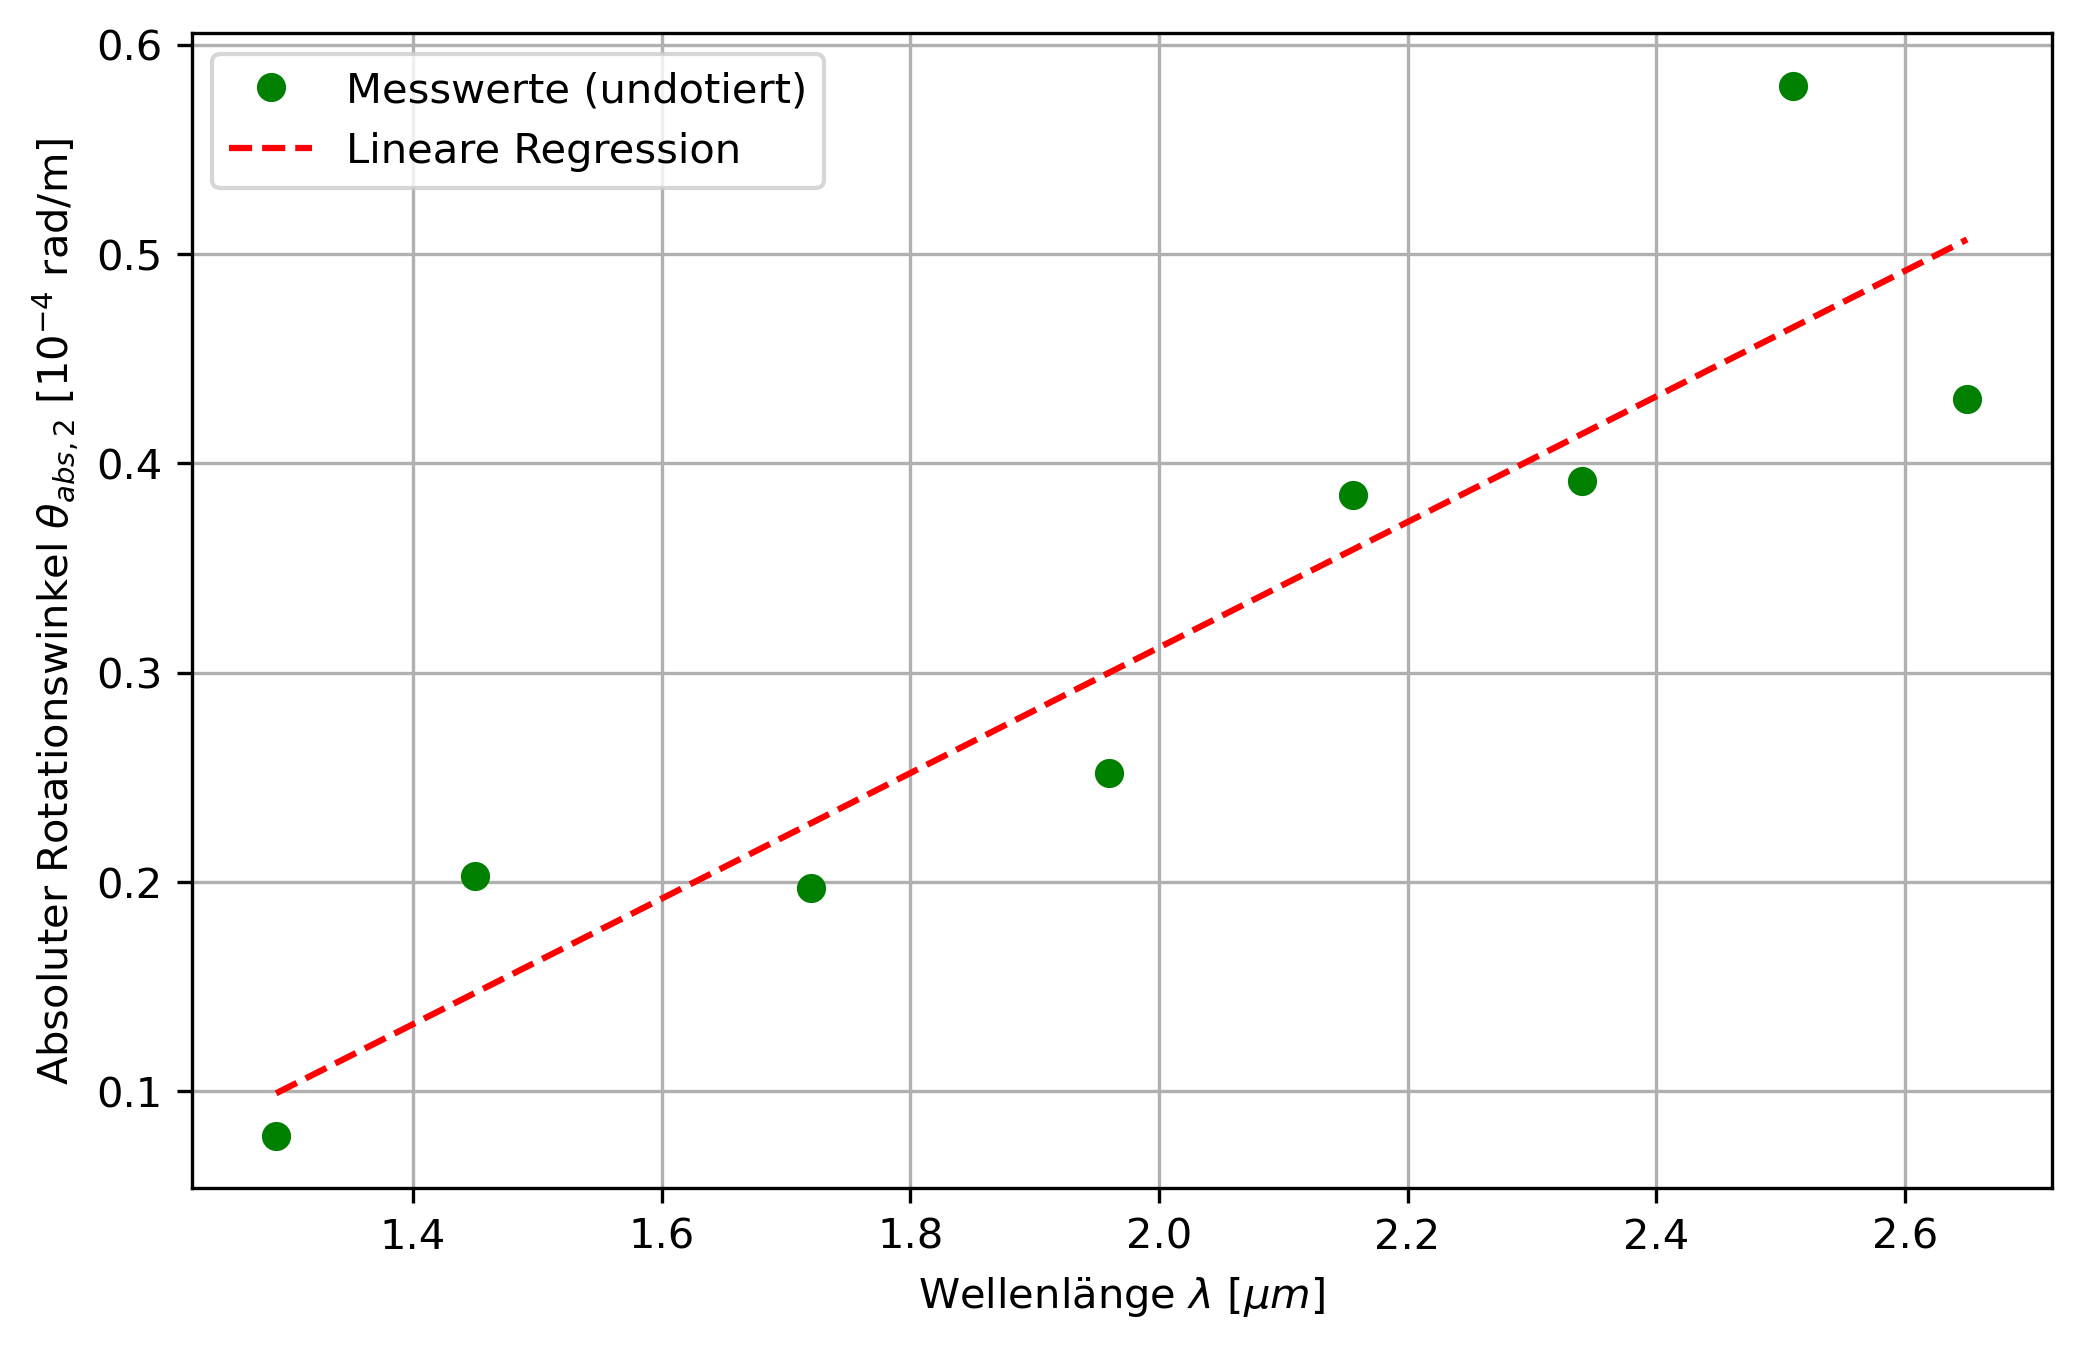
\includegraphics[width=0.8\textwidth]{content/plots/theta_abs_2_vs_lambda_linreg.png}
    \caption{Drehwinkel der Differenz der zweiten n-dotierten Probe in Abhängigkeit der Wellenlänge.}
\end{figure}
Die lineare Regression liefert für $y=a \cdot x + b$ den Wert
\begin{align*}
    a_2 &= \qty{3.00 \pm 0.51 e-5}{\per\micro\metre\cubed} \\
\end{align*}

Mithilfe von 
\begin{equation*}
    \begin{split}
        m^\ast &= \sqrt{\frac{e^3 \cdot N \cdot B}{8 \pi^2 \cdot \varepsilon_0 \cdot c^3 \cdot n \cdot a}} \\
    \end{split}
\end{equation*}
kann die effektive Masse $m*$ bestimmt werden.
Daraus folgt
\begin{align*}
    m_{\text{eff},1} &= \num{0.046 \pm 0.004} \, m_{\text{e}} \\
    m_{\text{eff},2} &= \num{0.036 \pm 0.003} \, m_{\text{e}}
\end{align*}
für die beiden effektiven Massen.
\clearpage
\section{Diskussion}
\label{sec:Diskussion}

Die relative Messabweichung wurde nach der Formel 
\begin{equation}
    \Delta x =   \frac{ \left| x_{exp} - x_{theo} \right|   }{x_{theo}}  
    \label{eq:abweichung}
\end{equation}
bestimmt.

\subsection{Bestimmung des B-Feldes}
Die Bestimmung des B-Feldes hat gut funktioniert, hierbei sind keine offensichtlichen Fehler aufgefallen.
\subsection{Bestimmung der effektiven Masse}
Um einen Vergleich zu ziehen, ob die Messung gelungen ist wird der Wert der effektiven Masse mit dem Theoriewert von GaAs verglichen. Hierzu folgt der Theoriewert von GaAs \cite{GaAs} mit 
\begin{equation*}
    m^\ast = 0.067 \, m_e.
\end{equation*}
Daraus ergibt sich nach \eqref{eq:abweichung} eine relative Messabweichung von 
\begin{align*}
    m_{\text{eff,1}} &= 31.34\,\% \\
    m_{\text{eff,2}} &= 41.79\, \%
\end{align*}
Der Fehler kann hierbei zustande kommen, wegen ungenauem Ablesen der Messinstrumente oder es kann der Polarisationfilter beispielsweise nicht perfekt eingestellt sein für die einzelnen Messungen. Ein weiterer Grund für den Fehler kann die Wärme des Magneten gewesen sein, welcher im Verlauf des Versuchs immer heißer geworden ist, wodurch die Leitfähigkeit des Halbleiters erhöht wird. 
Aufgrund von beispielsweise veralteter und fehlerbehafteter Messgeräte kann es des weiteren zu Fehlern kommen, so musste beispielsweise ein Messwert in \autoref{fig:masse2} in der linearen Regression ignoriert werden.
Was durch die Messung aber bestätigt werden konnte ist, dass die dichter dotierte Probe eine höhere effektive Masse hat als die weniger dicht dotierte Probe, was dadurch erklärt werden kann, dass bei GaAs die Bandstruktur einen großen Anharmonischen Anteil hat, sich die effektive Masse also stärker mit der Energie der Elektronen ändert und somit bei einer erhöhten Dichte von Leitungselektronen auch stärker von der weniger stark dotierten Probe abweicht.
\clearpage
\section{Anhang}
\label{sec:Anhang}

\begin{figure}[H]
    \centering
    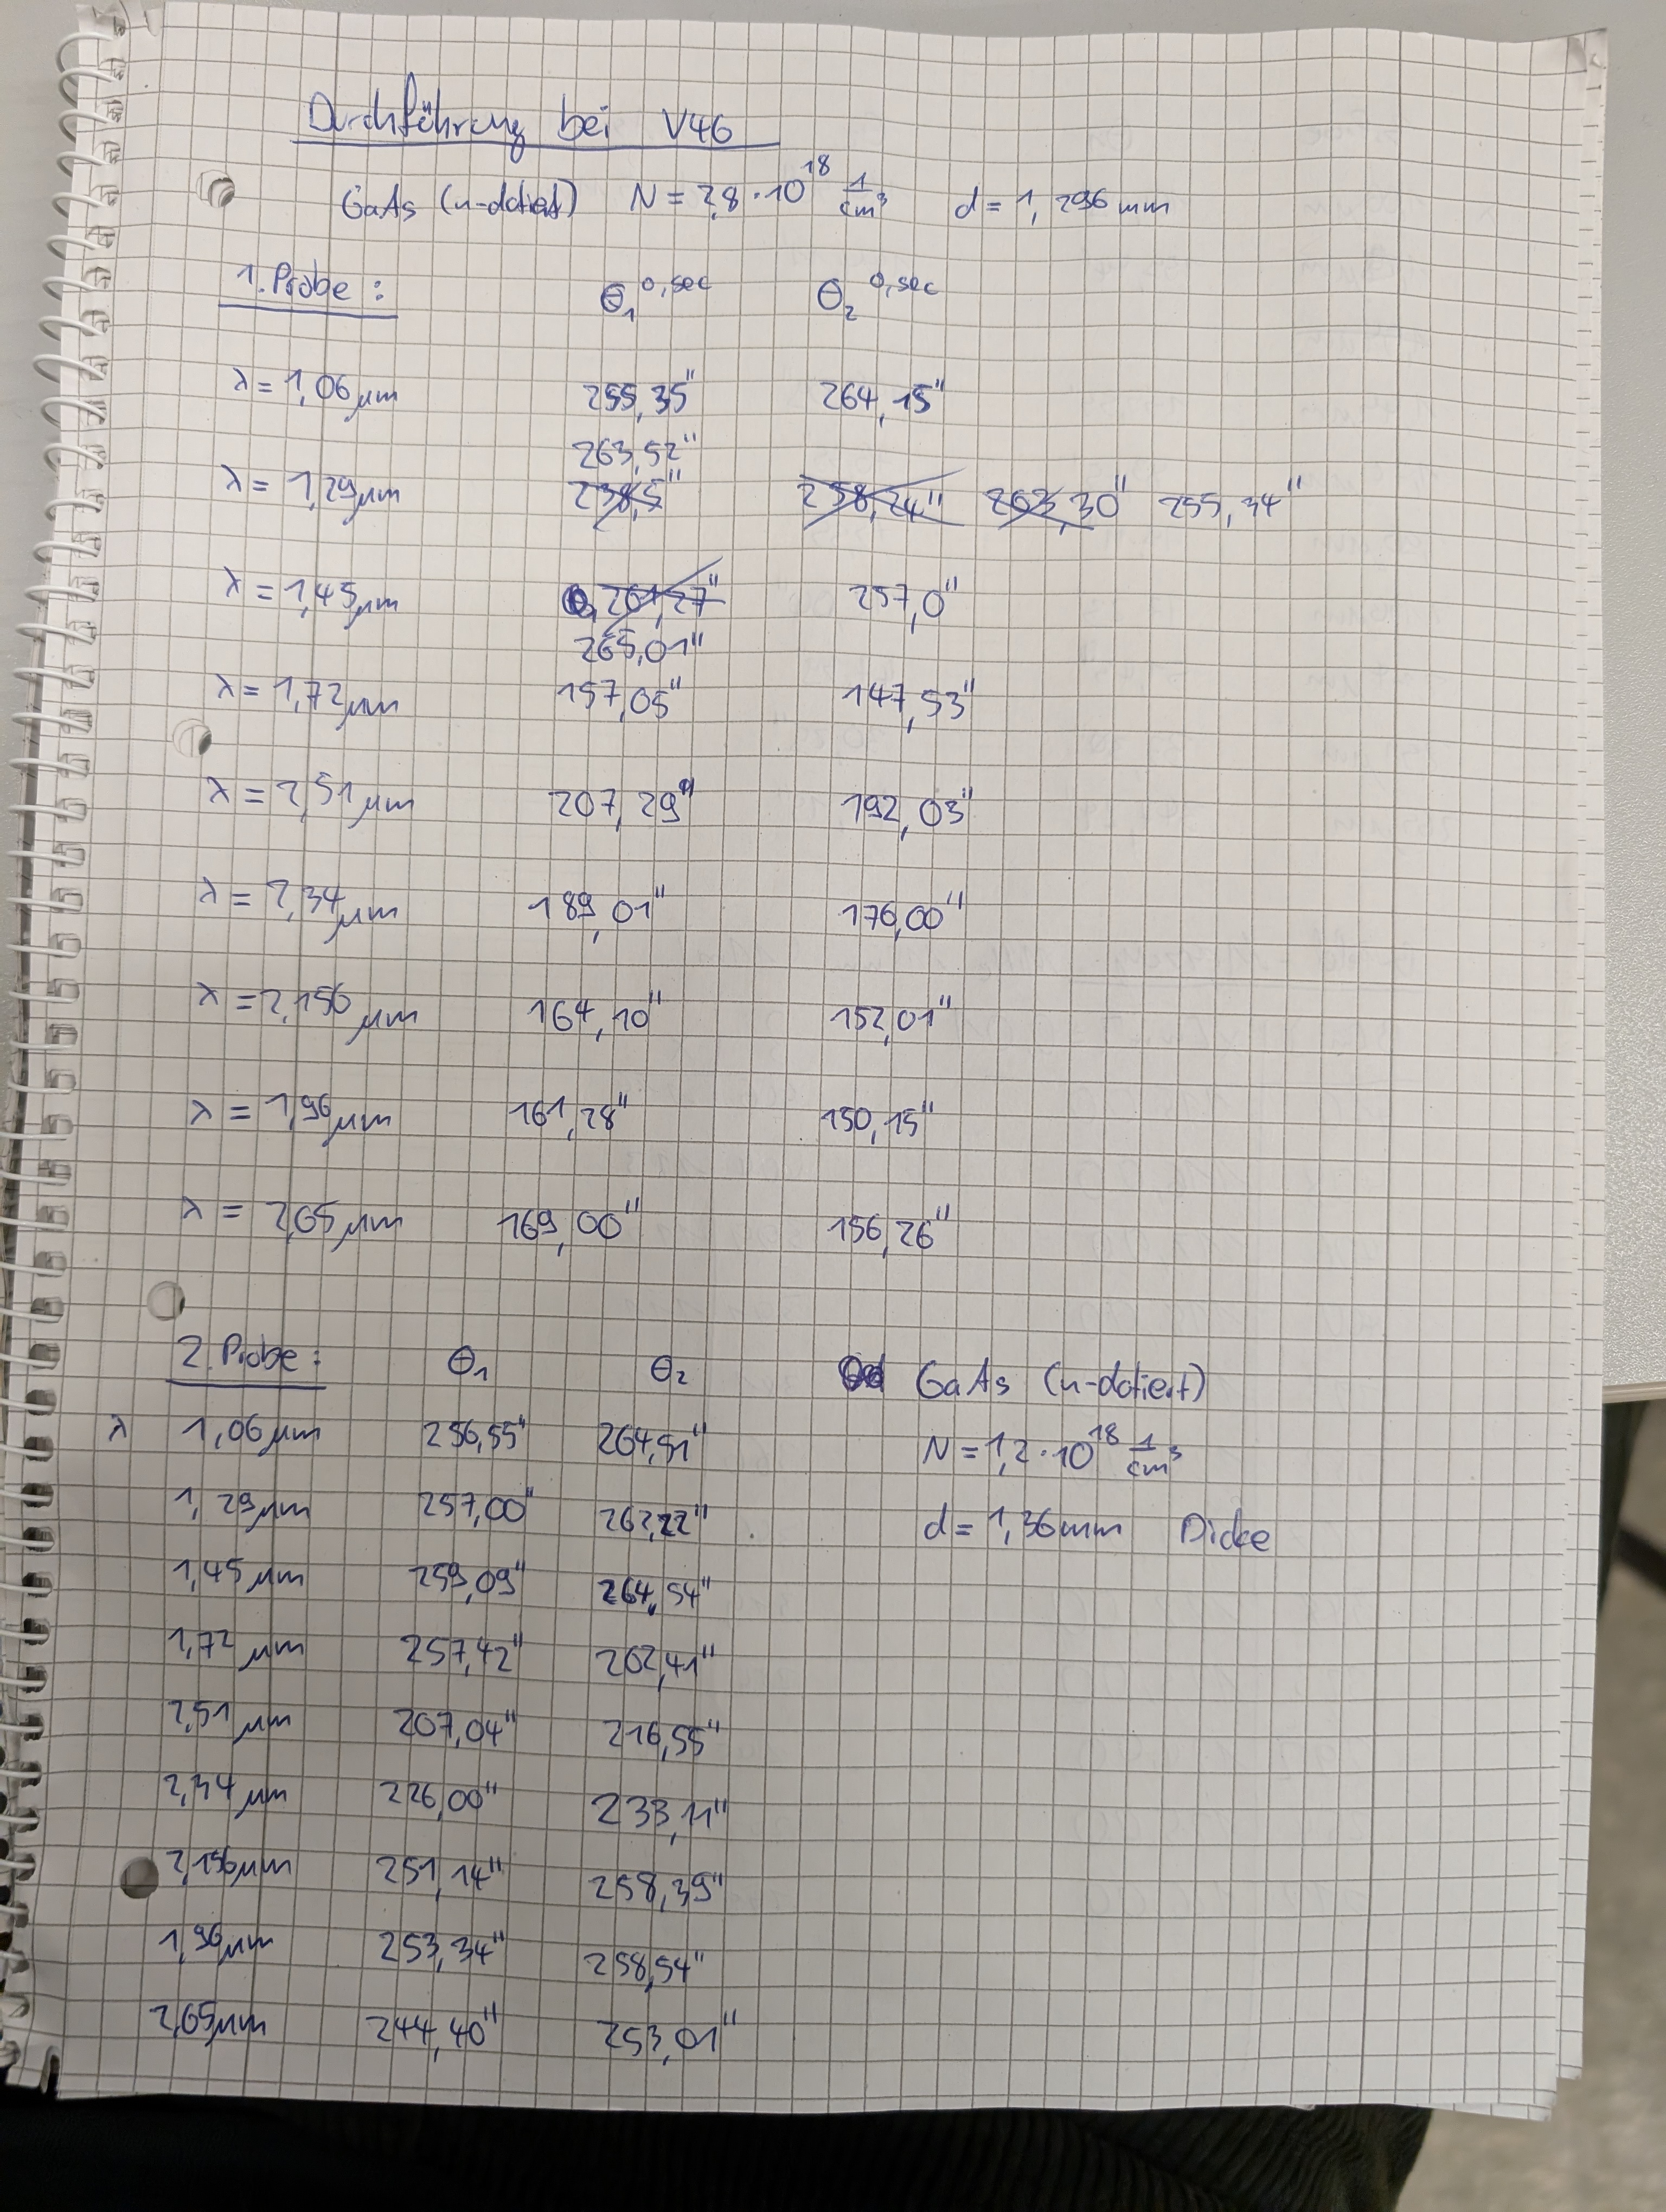
\includegraphics[width=0.4\textwidth]{content/pics/anhang1.jpg}
    \caption{Messwerte Seite 1.}
    \label{fig:anhang1}
\end{figure}

\begin{figure}[H]
    \centering
    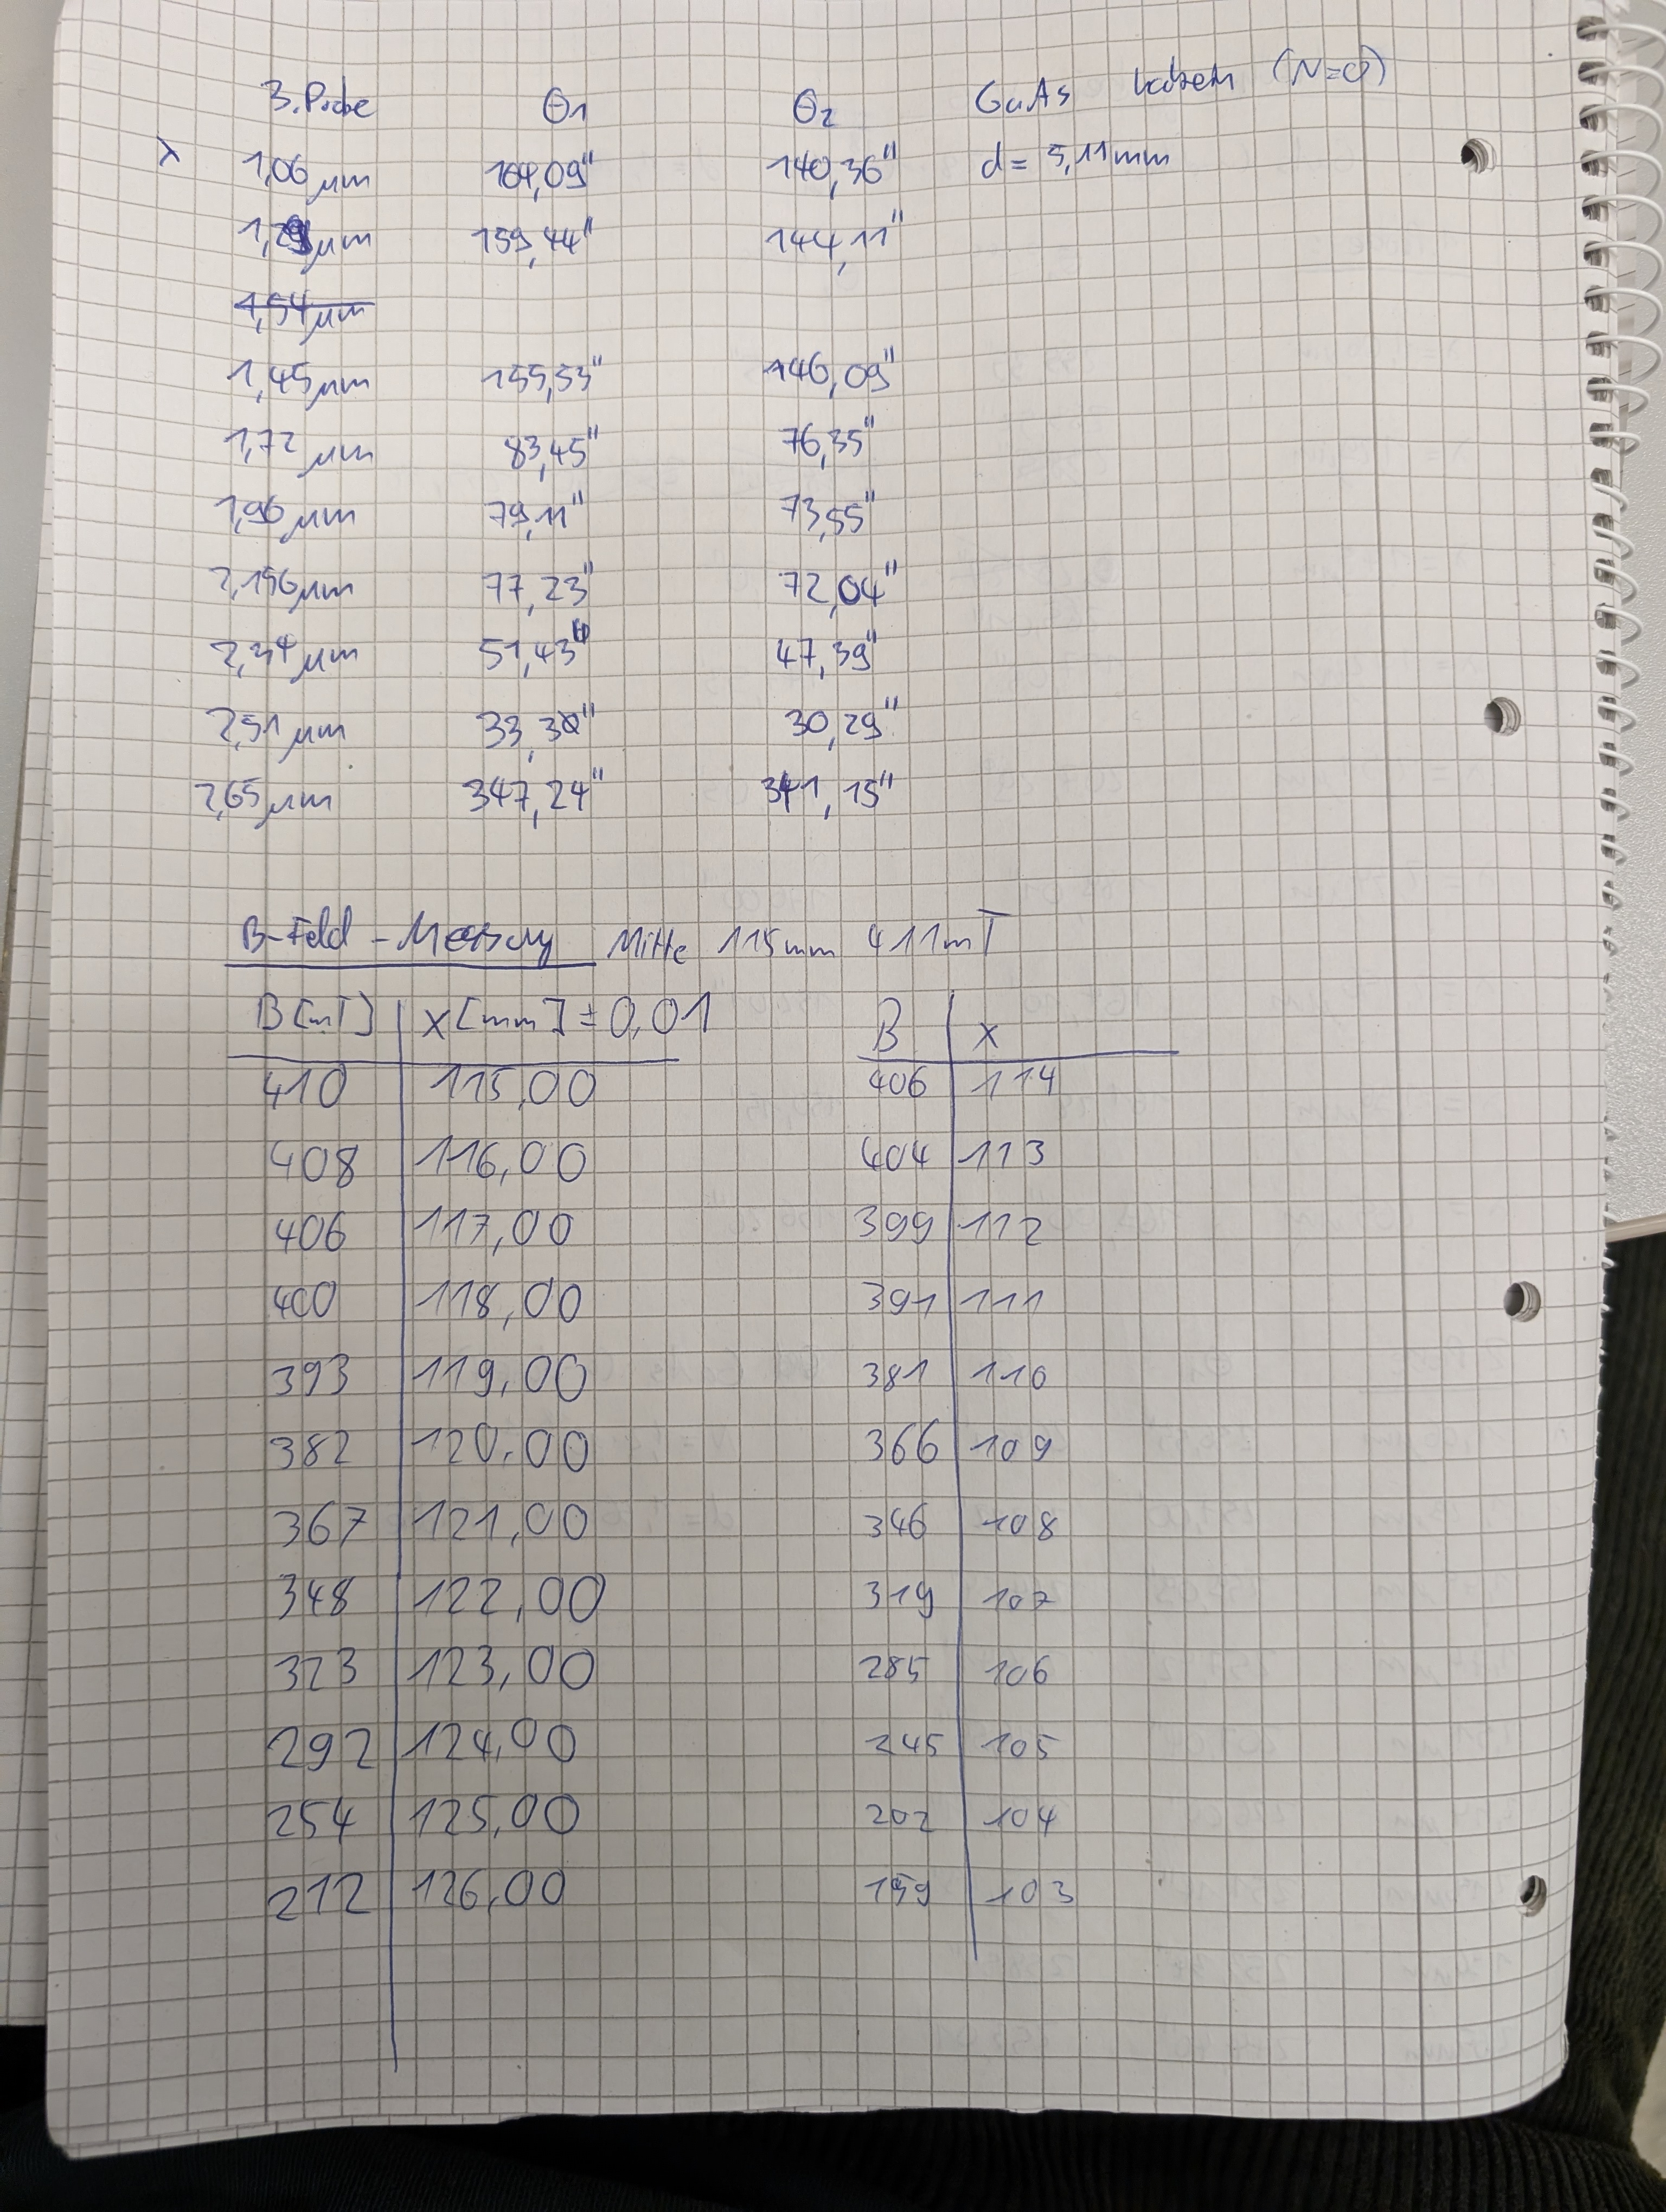
\includegraphics[width=0.4\textwidth]{content/pics/anhang2.jpg}
    \caption{Messwerte Seite 2.}
    \label{fig:anhang2}
\end{figure}
\clearpage

\printbibliography{}

\end{document}

